\subsection{Recent Developments}
\label{sub:dl_developments}

After basic paradigms of training neural networks were introduced in the last
subsection, this chapter dives deeper into more sophisticated approaches
which were developed in the last years of deep learning research.
Therefore, the first part explains the drivers behind current progress in the
field (ch.~\ref{sub:dl_drivers}). More complex network architectures which enable
broader practical application will be discussed afterwards (ch.~\ref{sub:dl_architectures}),
before the remaining sections describe modern approaches to optimization
(ch.~\ref{sub:dl_optimization_algos}) and regularization of the training process
(ch.~\ref{sub:dl_regularization}).

\subsubsection{Drivers}
\label{sub:dl_drivers}

Progress in deep learning research is mainly enabled by two factors, namely
increased data availability and improved hardware for computation.
Both factors will be detailed in the following.

\paragraph{Big data}

The term big data is used to describe the phenomenon of increased data
availability.
Main causes for this are migration of transactions from the physical world
to the internet, wide spread of mobile devices like smartphones and success
of social networks, e.g., \textit{Facebook} and \textit{Twitter}.
Big data can best be described by the three dimensions volume, velocity and
variety, also known as the \textit{Three V's}.
Here, \textbf{volume} describes increases in created data, mainly over the 
internet. 
Where volume refers to total size of data sets, \textbf{velocity} stands for the
speed-up in data access. More and more data can be consumed in (nearly) real-time,
e.g., over streaming interfaces.
In addition, big data comes in more diverse form, which is where the \textbf{variety}
dimension has to be regarded.
User-generated images and videos, as well as sensor or GPS data from smartphones
are examples for data types which complement more traditional text and relational
data.
Companies making use of big data in the form of data-driven decision making
have been shown to be more profitable and productive than companies that do not
apply such practices~\cite{McAfee2012}.
Modern world connectedness makes it possible to store data coming from
many different sources and process it in centralized manner, e.g., to offer
individualized services for consumers~\cite{Jordan2015}.
Deep learning profits from big data, particularly because models become more
precise with larger data sets.
Large data sets have been shown to improve model performance more than careful
feature engineering, which is required for most machine learning algorithms~\cite{Goodfellow2016}.
This trend is exemplified in growing benchmark data sets for deep learning
models.
For example, the \textit{MNIST} data set contains 70,000 images of size 28$\times$28 
pixels and served as a benchmark for image recognition since being first
introduced in 1998~\cite{LeCun1998}.
Nowadays, the most commonly used benchmark for the same task is the \textit{ImageNet}
database, which consists of about 1.2 million images in higher 
resolution~\cite{Russakovsky2015}.

\paragraph{Computational resources}

Processing larger data sets demands a higher number of necessary computations.
Hence, computational resources have to evolve in order to calculate models
in a timely manner.
Deep learning models are most commonly trained using \textit{graphics processing
units} (GPUs), which were formerly applied to highly parallelized processing
in computer games.
GPUs are preferred over CPUs for these tasks, because they contain more
processing units which can carry out computations in parallel.
Graphics processors enable training of more complex models, i.e., models which
contain more neurons and thus learn representation with higher numbers of 
parameters~\cite{Goodfellow2016, Raina2009}.

\begin{figure}[h]
  \centering
  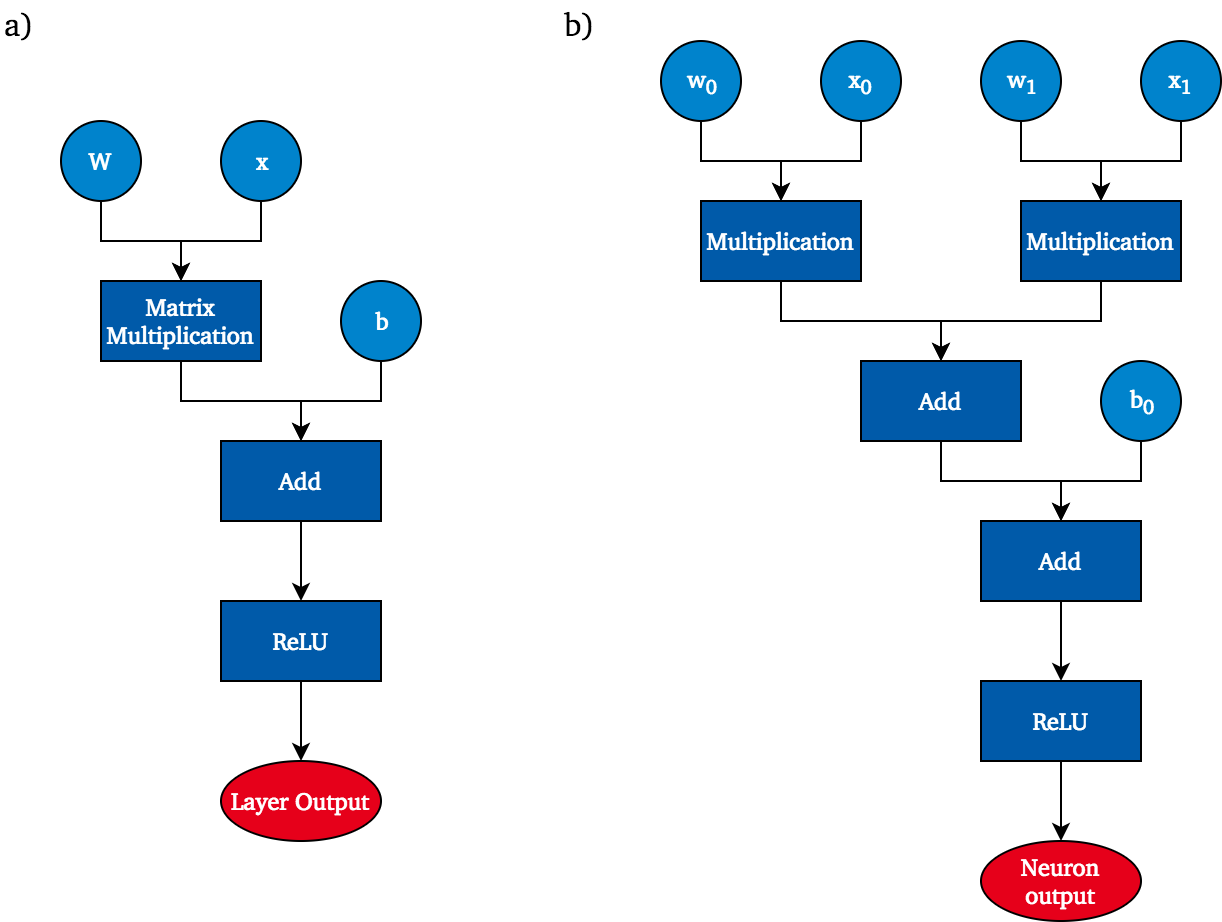
\includegraphics[height=10cm]{img/computation_graph_3}
  \caption[Computation graph for single layer and neuron]{Left: computation graph for a single layer \\ Right: computation graph for a single neuron}
\label{fig:comp_graph}
\end{figure}

Modern deep learning frameworks such as \textit{TensorFlow}\footnote{\url{https://www.tensorflow.org/}}
make use of GPUs by computing neuron outputs for a single layer in parallel.
Forward and backward propagation can be visualized using \textbf{computation
graphs}, which exemplify the single operations for calculating layer outputs.
Figure~\ref{fig:comp_graph}a shows a computation graph for the forward
pass through a fully-connected layer, as introduced in chapter~\ref{sub:dl_forward}.
Instead of computing the matrix operations on a single processing unit, the
calculation can be broken down into less complex subtasks.
Figure~\ref{fig:comp_graph}b exhibits the computation of a single neuron output
from a two-dimensional input vector $x$, which is obviously independent of
other activation computations in the same layer.
Most notably, matrix operations are replaced with element-wise calculations here.
Deep learning software typically computes forward and backward pass in this way
layer by layer in order to speed up the training process~\cite{Abadi2016}.

This work applies modern deep learning software and hardware for its model.
Exact specifications can be found in chapter~\ref{ch:methodology}.

\subsubsection{Network architectures}
\label{sub:dl_architectures}

Above described drivers enable training of more complex models for various
tasks.
In detail, these models contain more parameters and thus possess higher
representational capability.
Over decades of neural network reserach, specialized architectures have been
developed for tasks like image or speech recognition.
This subsection will present three network architectures, two of which will
be used for the model of this work.
For better understanding the architectures are compared to the basic fully-
connected model from chapter~\ref{sub:dl_concepts}

\paragraph{Convolutional neural networks (CNN)}

\begin{figure}[h]
  \centering
  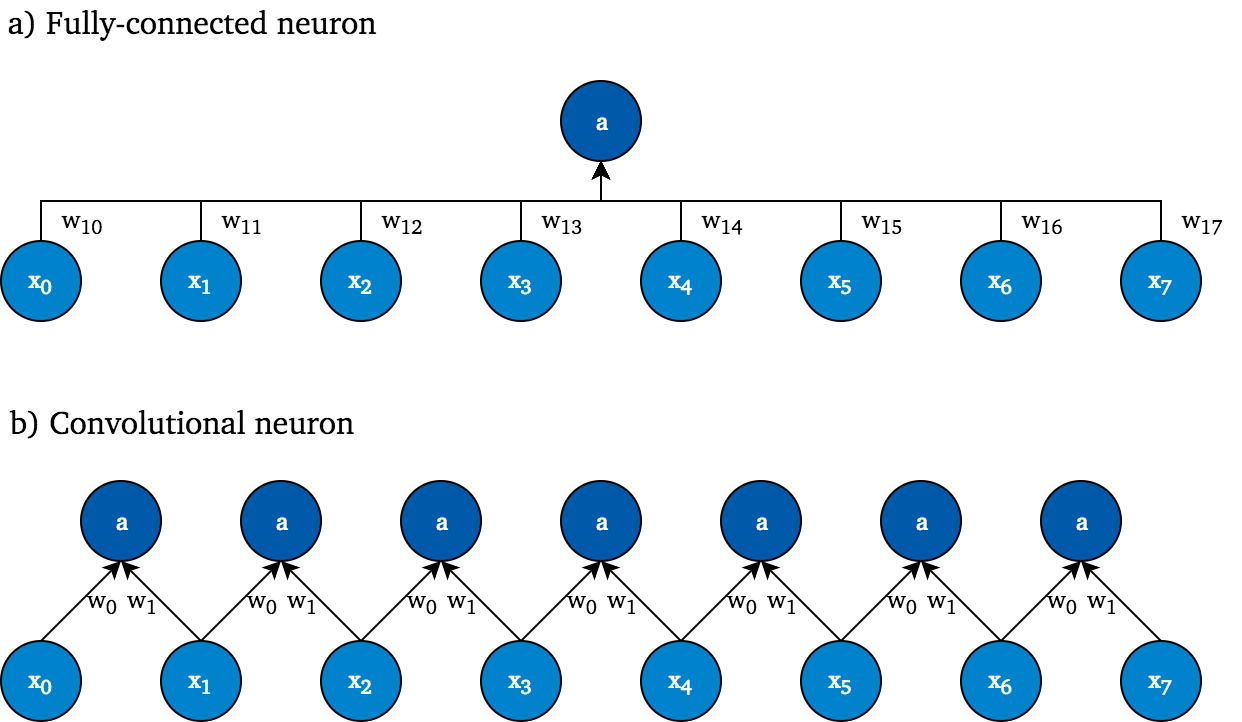
\includegraphics[height=8cm]{img/conv_layer.png}
  \caption{Comparison of fully-connected and convolutional neuron}
\label{fig:conv_layer}
\end{figure}

Convolutional neural networks were first developed by LeCun et al. in 1998,
based on approaches that had been invented during the 1980s~\cite{Fukushima1980, LeCun1998}.
At that time they were mostly used for simple image processing tasks like
automatic character recognition from handwriting.
In order to understand what characterizes convolutional layers, it is helpful
to compare them to fully-connected layers.
Figure~\ref{fig:conv_layer} compares both layer types for a one-dimensional
input vector and a single neuron in the network layer.
In a fully-connected layer, all inputs are connected to the same neuron.
Contrary, in a convolutional layer, a fixed number of neighboring inputs (two in this example)
are connected to a neuron copy.
All neuron copies share the same weights, as denoted in Fig.~\ref{fig:conv_layer}b,
and thus learn a shared representation of some pattern.
For convolutions to make sense, the ordering of inputs has to be relevant.
This is the case for several data types, e.g., image, text or speech data.
Images will be used as an example here, because the effects of applying
convolutions can be visualized.
Intuitively, one can imagine a convolution as a neuron that is moved over the
vector of inputs and looks for one specific pattern.
For images, a convolution can thus be thought of as a filter that represents
a common reoccuring visual theme.
What kind of pattern (also called \textit{filter}) is learned by the neuron is
determined during the training process.

\begin{figure}[h]
  \centering
  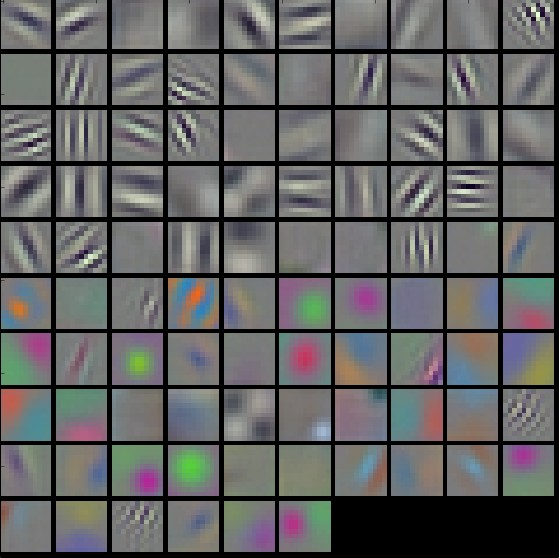
\includegraphics[height=8cm]{img/conv_filters.jpeg}
  \caption[Example filters in a convolutional layer]{Example filters in a convolutional layer~\cite{Krizhevsky2012}}
\label{fig:conv_examples}
\end{figure}

Figure~\ref{fig:conv_examples} shows examples for such filters, as found in
a large convolutional neural network~\cite{Krizhevsky2012}.
The top half of filters identify edges of varying orientation and thickness,
whereas the bottom half of filters focuses on color contrasts.
These are examples for filters learned in the first convolutional layer of a
network, that set a new benchmark for image recognition tasks.

\begin{figure}[h]
  \centering
  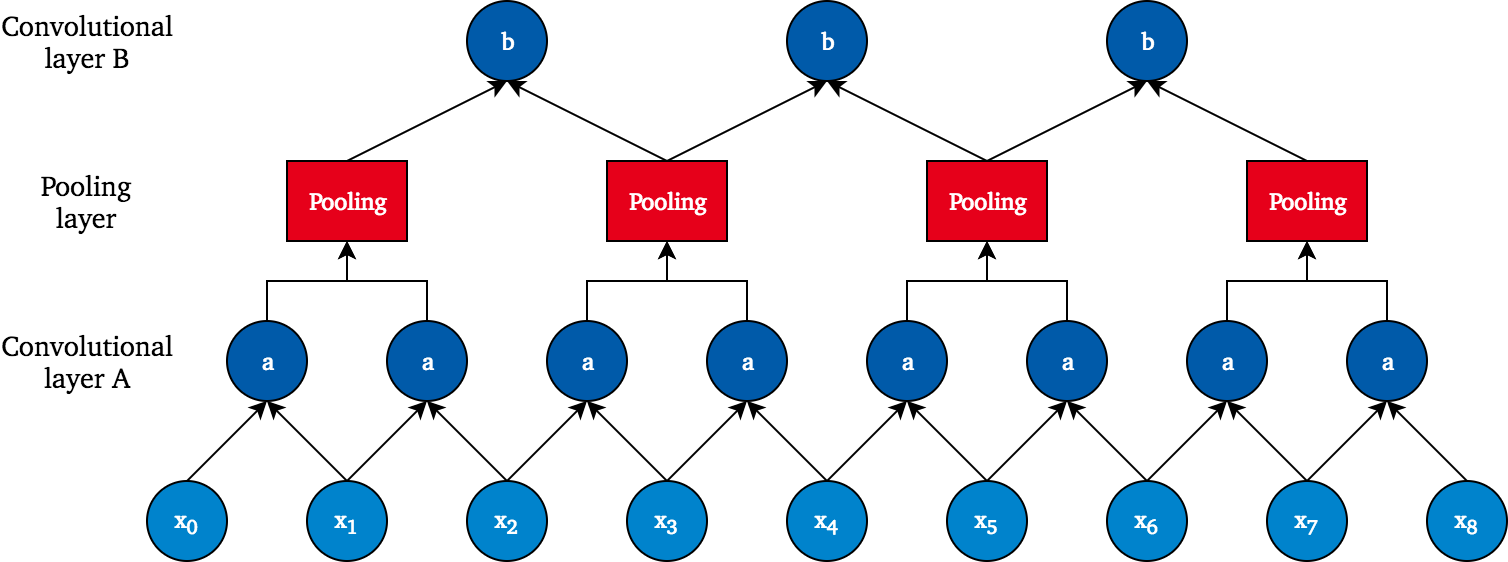
\includegraphics[height=6cm]{img/conv_architecture}
  \caption{Convolutional neural network}
\label{fig:cnn_architecture}
\end{figure}

In practice, convolutional layers are stacked, so that later layers can learn
to identify increasingly complex shapes, e.g., faces or objects, from more
primitive shapes like edges and color contrasts~\cite{Simonyan2015}.
\textit{Pooling layers} are often used to combine the output of neuron copies, which
enables the next convolutional layer to detect shapes from a greater portion of
the image effectively.
This effect is visualized in Fig.~\ref{fig:cnn_architecture}, where the first
neuron copy of layer $B$ learns a filter from the output of two neuron copies
of layer $A$.
As an example, if layer $A$ learns to detect a horizontal edge, layer $B$ can
find occurrences of two parallel edges in an image.

As mentioned before, convolutional neural networks are mostly applied to data
like images and texts.
More detailed practical applications will be discussed in chapter~\ref{sub:dl_applications}.

\paragraph{Recurrent neural networks (RNN)}

Like convolutional neural networks, recurrent neural networks (RNNs) are usually
used on data that underlies some kind of ordering.
Popular applications of RNNs lie in the  area of \textbf{Naturual Language
Processing (NLP)}, because text can be formalized as an ordered sequence of
words.

\begin{figure}[h]
  \centering
  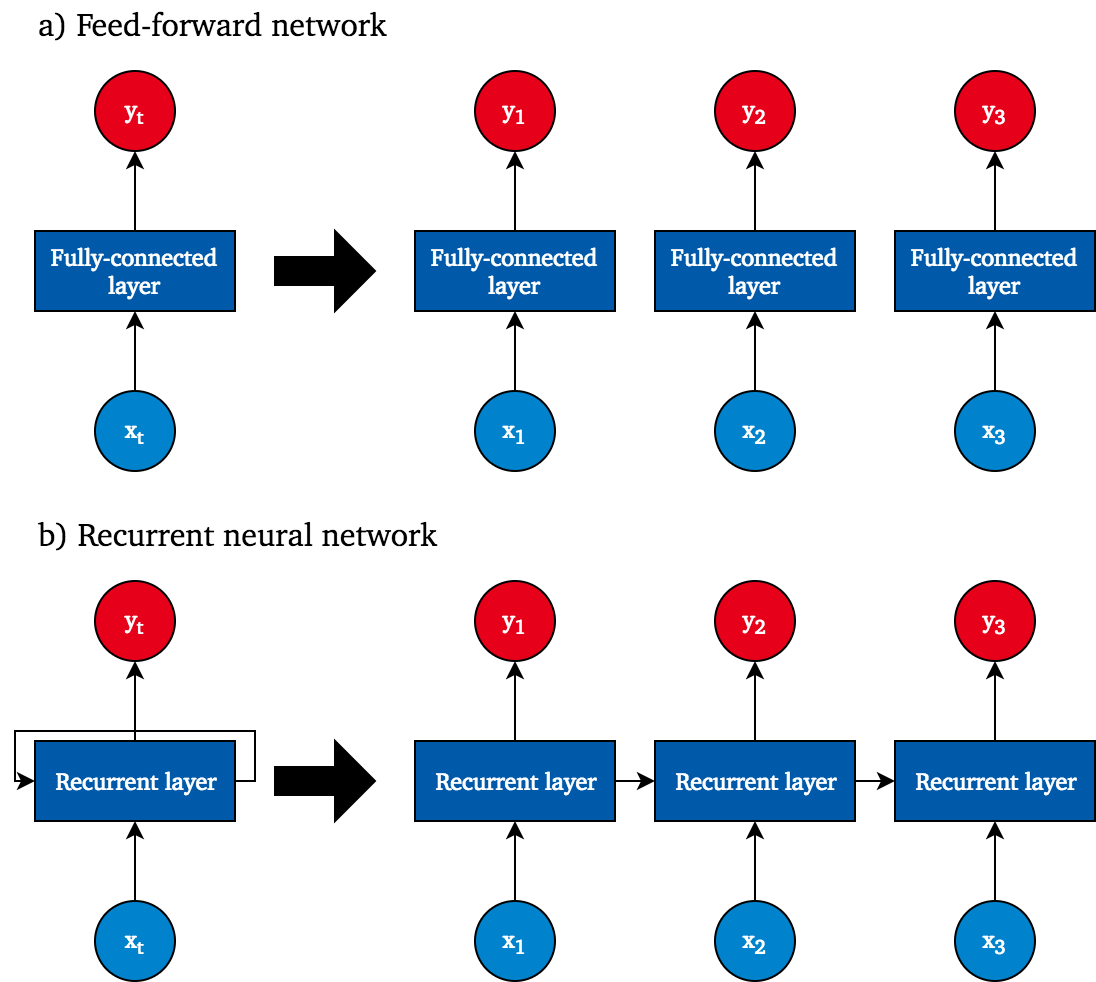
\includegraphics[height=10cm]{img/rnn_unrolled_2}
  \caption{Comparison between unrolled feed-forward and recurrent neural network}
\label{fig:rnn_unrolled}
\end{figure}

One drawback of basic feed-forward networks (see chapter~\ref{sub:dl_concepts})
when looking at ordered sequences is the lack of persistence between single
iterations.
Thus, when looking at an example $x_t$ the network does not know about previous
examples, e.g., $x_{t-1}, x_{t-2},\cdots$.
This fact is exemplified in Fig.~\ref{fig:rnn_unrolled}a, which unrolls a
feed-forward network containing one fully-connected layer into single iterations.
Intuitively, knowing about formerly observed events is useful in many use cases,
e.g., translation tasks or time-series forecasting.
Recurrent neural networks overcome the liability by introducing the concept
of \textbf{memory}.
As shown in Fig.~\ref{fig:rnn_unrolled}b, information is passed between
iterations, which for example enables the network to memorize previous inputs~\cite{Goodfellow2016}.
The most applied RNN variant is the so-called \textbf{Long Short-Term Memory}
network, which will be explained in the following.

\begin{figure}[h]
  \centering
  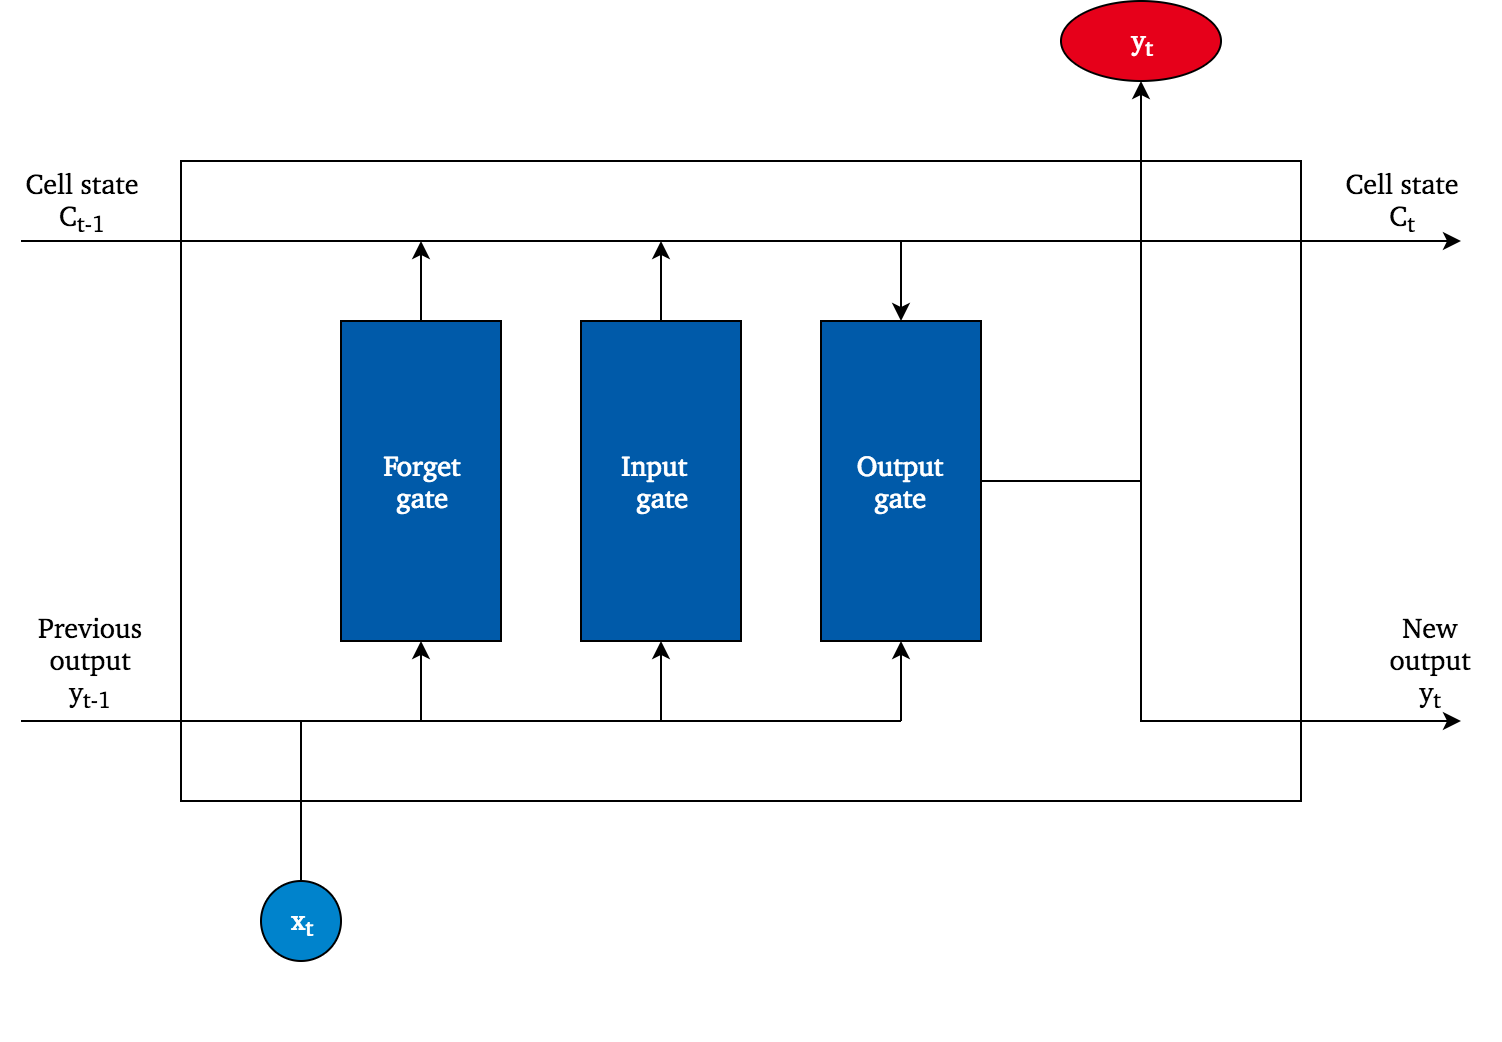
\includegraphics[height=11cm]{img/lstm_cell}
  \caption{Simplified LSTM cell}
\label{fig:lstm_cell}
\end{figure}

The Long Short-Term Memory (LSTM) network was first introduced by Hochreiter \&
Schmidhuber~\cite{Hochreiter1997} in 1997, aiming to solve the problem of
storing information in a neural network over time.
A LSTM neuron (often calledLSTM cell) comprises four separate layers which 
manipulate the \textit{cell state}.
The cell state stores information and is passed between iterations of the
training process.
In summary, the four included layers serve three purposes: removing unnecessary
information, adding new information and creating an output.
The three tasks are handled in \textit{gates} which contain the necessary
network layers for computation and are responsible for editing the cell state
accordingly.
The following explanations of LSTM gates are illustrated in Fig.~\ref{fig:lstm_cell}.

All three gates process the current input $x_t$ and the output of the previous
iteration $y_{t-1}$.
LSTMs are commonly applied for Natural Language Processing tasks such as
language modeling, i.e., prediction of the next word based on previously seen
text.
Therefore, an example language modeling task will be used to describe the
gate functionalities~\cite{Olah2015}.
Firstly, the \textit{forget gate} decides which information can be removed from
the cell state.
Internally, the forget gate contains a simple layer with sigmoid activations.
Outputs of the layer are multiplied element-wise with the cell state.
The activations are guaranteed to be between zero and one, where zero represents
`forgetting' and one stands for `keeping' information.
For example, when trying to predict words in a sequence it is necessary
to know about the current subject in order to conjugate an upcoming predicate
correctly.
If the current input $x_t$ represents a new subject, e.g., `he',the old subject should
probably be removed from the cell state in the forget gate.
Secondly, the \textit{input gate} is responsible for adding new information to the cell
state.
It does so in two distinct steps, which are processed in separate layers.
Here, the first decision is which information to update, and the second one
which new values to add.
The layer outputs are combined using the Hadamard Product and then added to the
cell state.
Continuing previous example, the input gate would likely add information about
the gender of the new subject, which determines word endings for predicates in
many languages.
Finally, an output for the current iteration is generated in the \textit{output gate}.
The output represents `a filtered version'~\cite{Olah2015} of the cell state, e.g.,
information for upcoming verbs when a new subject is observed.
This happens through the use of another layer with sigmoid activations which
intuitively filters relevant information from the cell state.
As can be seen in Fig.~\ref{fig:lstm_cell}, the output is also passed to the
next iteration.

LSTMs have been applied to problems ranging from speech recognition to
image captioning, which require storing input information with regard to the
training process.
Architectures using multiple, stacked LSTM layers are also used in practice,
mainly to learn even more complex representations.
Detailed use cases will be a central theme in Ch.~\ref{sub:dl_applications}.

\paragraph{Generative adversarial networks}

The previously described architectures of CNNs and RNNs were developed prior to
the third wave of neural network research and became efficiently trainable
due to driving factors described in Chapter~\ref{sub:dl_drivers}.
Finally, this subsection introduces \textit{Generative Adverserial Networks (GANs)}, which
represent a more recently invented model architecture.
The basic concept was presented by researchers in 2014, and has gained popularity
since then~\cite{Goodfellow2014}.
As can be extracted from the name, GANs belong to the family of \textit{generative
models}.
In contrast to \textit{discriminative models} which learn a decision boundary
between classes (e.g., Support Vector Machines), generative models implicitly 
model the probability distribution of inputs and outputs~\cite{Bishop2006}.
Therefore, generative models can be used to generate new data from the learned
distribution, e.g., new images can be created from a sample of real images.
Generative adversarial networks approach this problem by combining two neural 
networks into a single model, as illustrated in Fig.~\ref{fig:gan_architecture}.

\begin{figure}[h]
  \centering
  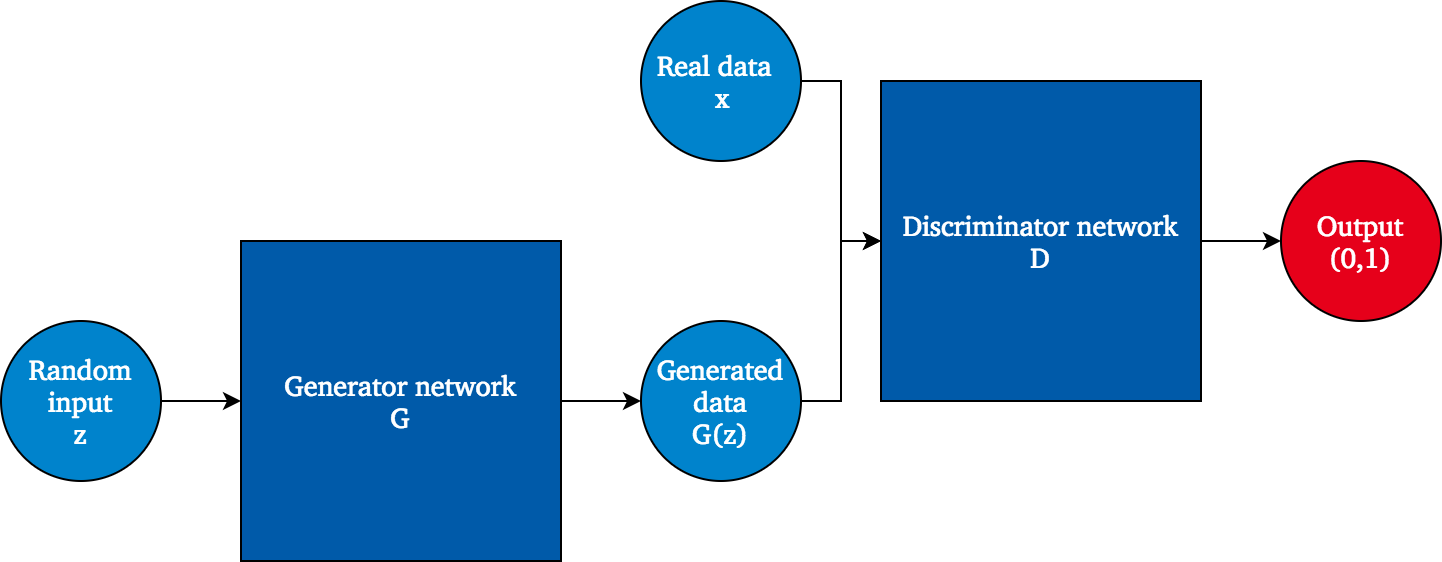
\includegraphics[height=6.5cm]{img/gan_architecture}
  \caption{Architecture of a Generative Adversarial Network (GAN)}
\label{fig:gan_architecture}
\end{figure}

In general, a GAN consists of a \textit{generator network G} and a \textit{discriminator network D}.
The generator outputs new data $G(z)$ from a random input vector $z$ which is
drawn from a normal distribution.
The generated data then serves as an input to the discriminator, along with
real data $x$.
Tasked with distinguishing between real and generated data, the discriminator
outputs probabilities representing an estimation of the authenticity of an
example.
Intuitively, the aim of the GAN architecture is to create new samples that carry
such similarity with original samples, that the discriminator can not differentiate
between real and generated anymore.
The question arises, how this objective can be expressed in a cost function.
Traditionally, generative models were trained by minimizing the distance of
generated output to nearest sample in the real data~\cite{Goodfellow2014}.
GANs use a different objective function, which is exemplified in equation~\ref{eq:gan_obj}.

\begin{equation}
  \label{eq:gan_obj}
  \min_G \max_D V(D, G) = \mathbb{E}_{x \sim p_{data}(x)}[\log D(x)] + \mathbb{E}_{z \sim p_z (z)}[\log (1 - D(G(z)))]
\end{equation}

The cost function includes the objectives of both networks, as the generator
tries to minimize the above equation and the discriminator aims to maximize it.
Both terms represent in the equation represent log-likelihood functions.
Maximizing the equation means assigning the correct labels to data samples (aim
of the discriminator), minimizing it implies that the discriminator is not capable
of specifying where a sample comes from (aim of the generator).
The authors of the original paper prove the existence of a unique solution, where
the generator is able to represent the original data distribution and the 
discriminator outputs probabilities of 0.5 for every sample~\cite{Goodfellow2014}.
Such a game between two entities following conflictive objectives is referred to
as a \textit{minimax setting}~\cite{Russell1995}.

During the training process, weights for both networks have to be updated.
This can be achieved through backpropagating errors through both networks,
although some adaptations have to be made.
Training processes as follows:

\begin{enumerate}
  \item Determine architecture for generator and discriminator network
  \item Update $D$ while $G$ is not trainable and samples are split between real and generated
  \item Update $G$ while $D$ is not trainable and samples are all generated
  \item Repeat steps 2 and 3 for desired number of iterations
\end{enumerate}

It becomes obvious that the two networks are updated alternatively.
An important caveat is that one network is not trainable, i.e., the weights are
fixed, while the other one is updated.
Fixed weights are not updated during training, but solely used to pass information
forward and backward through the network.

GANs were applied to creation of images in the original paper, but have been
used for a bigger variety of problems since. As for the other architectures,
more practical applications can be found in Ch.~\ref{sub:dl_applications}.
After examining more advanced architectures, the next two subsections will
focus on the training process.
In particular, developments in optimization algorithms and regularization
techniques are described.

\subsubsection{Optimization algorithms}
\label{sub:dl_optimization_algos}

The choice of optimization algorithms influences the stability of the training
process.
Here, the aim is to converge to a good solution in reasonable time, ideally
finding a minimum for the cost function by adapting weights in the network.
Chapter~\ref{sub:backprop} introduced a basic structure for optimization
algorithms in neural network training, as well as update functions for the
\textit{stochastic gradient descent} optimization algorithm.
Basically, gradient descent only relies on derived gradients and a hyperparameter
representing the learning rate, i.e., the step size towards a possible minimum
(~\ref{eq:gd}).
For complex neural networks, gradient descent can be hard to utilize effectively.
Suitable, often manual weight initialization and adaptions of the learning rate
during training are needed in order to derive good solutions.
More sophisticated optimization algorithms, which were developed in the last
years, overcome these limitations.
This subsection will first introduce the concept of \textit{momentum} in
numerical optimization and then explain a commonly deployed algorithm called
\textit{Adam}.

\begin{equation}
  \label{eq:gd}
  w_{t+1} \rightarrow w_t - \eta \nabla f(w_t)
\end{equation}

\paragraph{Momentum}

The concept of momentum was developed in the 1960s and has since been applied
to numerical optimization problems~\cite{Polyak1964}.
During the third wave of neural network research, the concept was first
utilized for accelerating training processes in deep networks~\cite{Sutskever2013}.
In its essence, momentum (equation~\ref{eq:momentum}) adds an additional step to 
the gradient descent update function (equation~\ref{eq:gd}).

\begin{align}
  \label{eq:momentum}
  v_{t+1} \rightarrow \mu v_t + \eta \nabla f(w_t) \\
  w_{t+1} \rightarrow w_t - v_{t+1}
\end{align}

The weight update $v_{t+1}$ is composed by two terms: the gradient $\nabla f(w_t)$
weighted with the learning rate $\eta$ and the previous update $v_t$ multiplied
with the \textit{momentum coefficient} $\mu$.
Therefore, the update in iteration $t+1$ depends on the update of iteration $t$,
which again is dependent on $v_{t-1}$ and so on.
The added term $\mu v_t$ can thus be interpreted as an exponentially moving 
average of previous updates, where hyperparameter $\mu$ determines the magnitude 
of influence of these predecessor updates.
Momentum allows the optimizer to progress more evenly without too many changes
of direction.
This overcomes the liability of gradient descent which is susceptible to
frequent changes of directions in the gradient, e.g., if examples in a mini-batch
are particularly noisy.

\paragraph{Adam}

As outlined in above paragraph, momentum keeps track of the exponentially moving
average of previous gradients.
This added average constitutes a first moment estimate of the gradients, also 
known as \textit{mean estimate}.
The \textit{adaptive moment estimation (Adam)} optimization algorithm enhances
momentum with further computations in order to guarantee accelerated
convergence~\cite{Kingma2014a}.
Intuitively, Adam adapts the learning rate for each parameter based on mean and
variance of recent updates in the specific parameter.
Equations~\ref{eq:adam_start} through~\ref{eq:adam_end} exemplify the update
computation for a single parameter $w$ in iteration $t$.

\begin{align}
  g_t &= \nabla f(w_t) \label{eq:adam_start} \\
  m_t &= \beta_1 m_{t-1} + (1-\beta_1) g_t \label{eq:adam_2} \\
  v_t &= \beta_2 v_{t-1} + (1-\beta_2) g_t^2 \label{eq:adam_3} \\
  \widehat{m}_t &= \frac{m_t}{1-\beta_1^t} \label{eq:adam_4} \\
  \widehat{v}_t &= \frac{v_t}{1-\beta_2^t} \label{eq:adam_5} \\
  w_{t+1} &= w_t - \frac{\eta}{\sqrt{\widehat{v}_t} + \epsilon} \widehat{m}_t \label{eq:adam_end}
\end{align}

Equations~\ref{eq:adam_2} and~\ref{eq:adam_3} compute mean and
uncentered variance estimates of the gradient, similar to momentum.
$\beta_1$ and $\beta_2$ are hyperparameters, whose default values are $0.9$ and
$0.999$ respectively.
Because of these defaults and zero initialization of $m$ and $v$, the estimates
are biases towards zero, especially in early iterations.
This bias is corrected in equations~\ref{eq:adam_4} and~\ref{eq:adam_5}, where
the scaling factor $\frac{1}{1-\beta_1^t}$ is larger for smaller values of $t$
and therefore accounts for smaller values of the estimates as a result of 
zero initialization.
Final updates are then calculated via the corrected estimates and hyperparameters
$\eta$ (representing the learning rate) and $\epsilon$ (defaults to $10^{-8}$).

\begin{figure}[h]
  \centering
  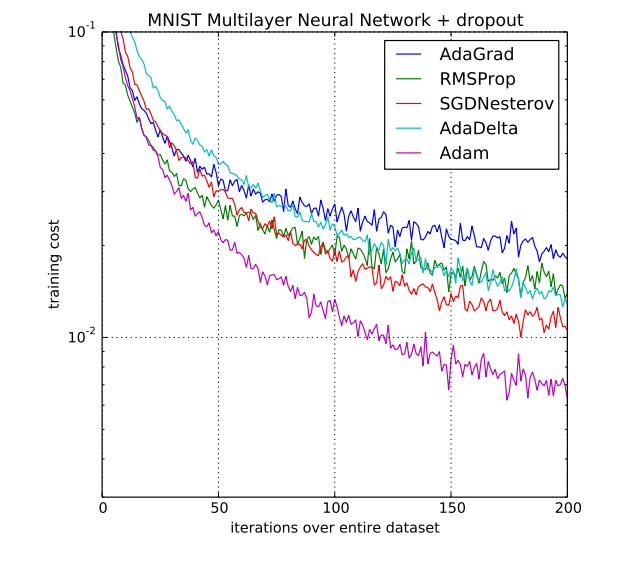
\includegraphics[height=10cm]{img/adam_comparison}
  \caption[Comparison of optimization algorithms]{Comparison of optimization algorithms~\cite{Kingma2014a}}
\label{fig:adam_comp}
\end{figure}

Kingma \& Ba~\cite{Kingma2014a} list concise implementation, computational efficiency,
suitability for complex models with many parameters and reasonable default values
for the hyperparameters as main benefits of adaptive moment estimation.
Figure~\ref{fig:adam_comp} compares Adam to other optimization algorithms,
applied in the context of a deep neural network with the task of handwriting
recognition.
It can be seen that Adam achieves a better solution, i.e., lower value of the
cost function, over the course of 200 iterations.

\subsubsection{Regularization techniques}
\label{sub:dl_regularization}

In addition to optimization algorithms, regularization techniques largely
influence training process stability and generalization ability of the
resulting model.
These techniques are particularly helpful for complex models such as deep
neural networks, and custom methods have been developed during the current
research wave.
This subsection will introduce regularization procedures after firstly explaining
the concept of overfitting which many techniques aim to prevent.

\paragraph{Overfitting}

\textit{Generalization} constitutes the main challenge in machine learning and
denotes the ability to `perform will on new, previously unseen inputs'~\cite[p. 110]{Goodfellow2016}.
Therefore, machine learning models should not only be evaluated using training
error, i.e., the performance measure on training data, but also via \textit{test
error}, i.e., the performance on unseen test data.
In summary, key objectives of machine learning algorithms can be put as follows:

\begin{enumerate}
  \item Minimize training error
  \item Minimize gap between training and test error
\end{enumerate}

\begin{figure}[h]
  \centering
  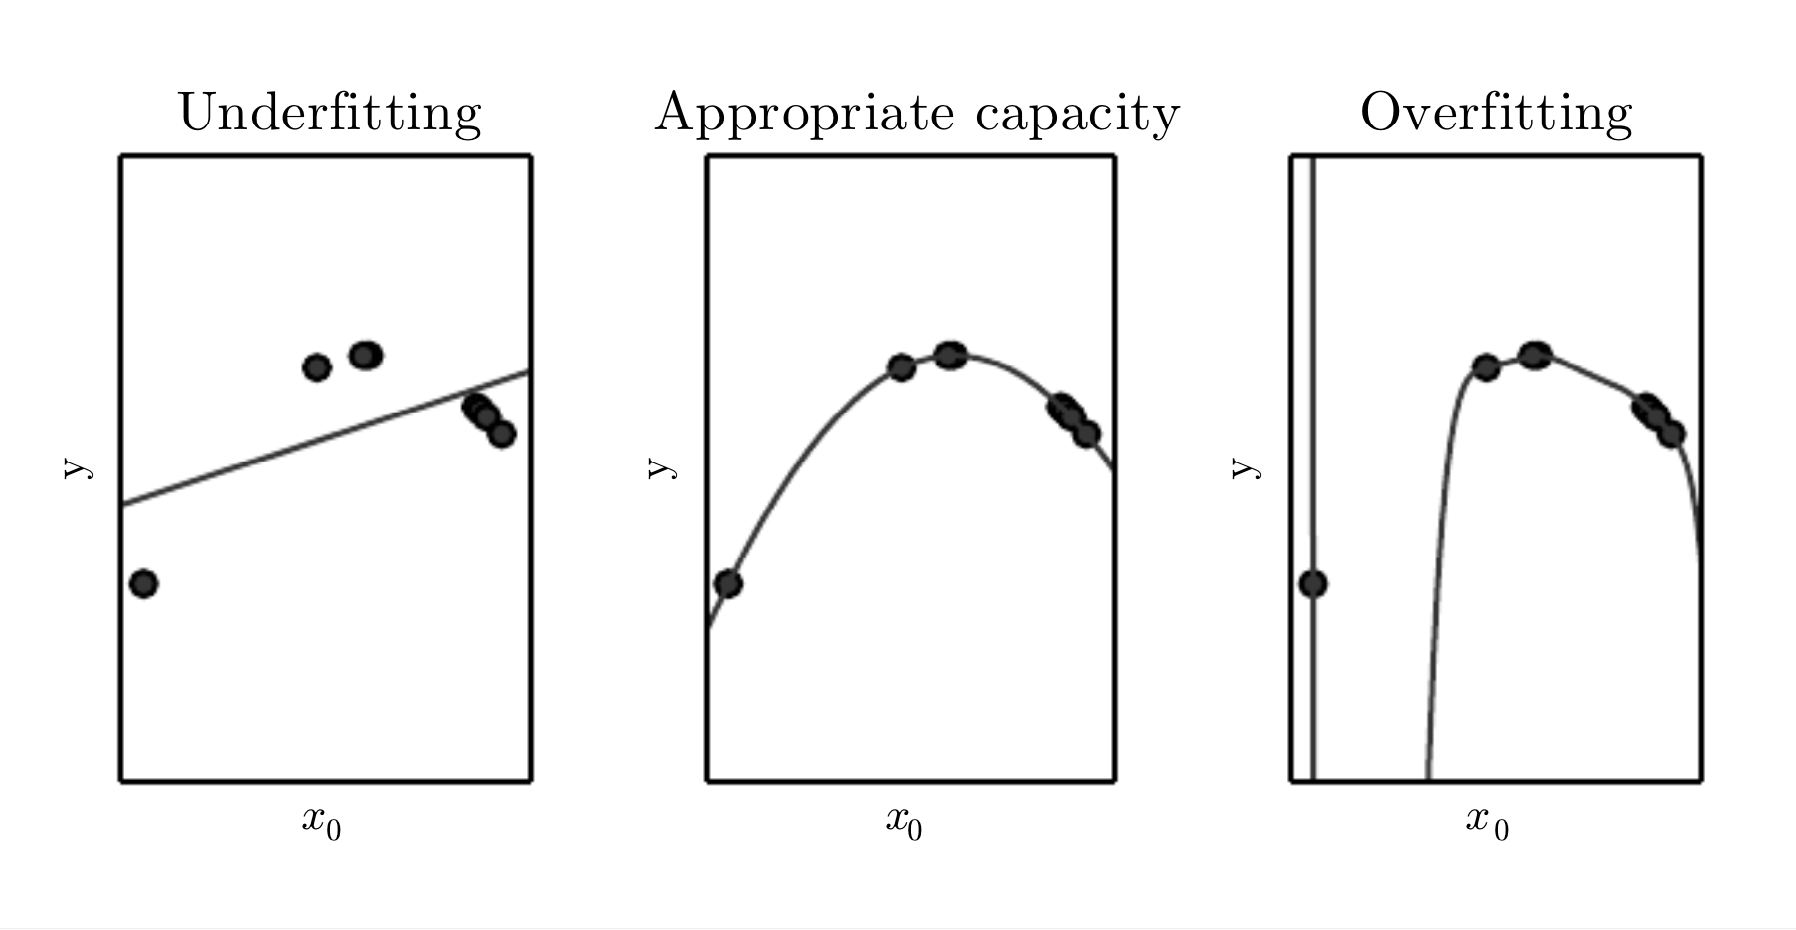
\includegraphics[height=8cm]{img/overfitting}
  \caption[Overfitting, underfitting and appropriate capacity]{Overfitting, underfitting and appropriate capacity~\cite{Goodfellow2016}}
\label{fig:overfitting}
\end{figure}

\textit{Overfitting} simply refers to a large gap between training error and test
error.
Intuitively, the model learns too much about specific examples in the training
set and can not perform well on other data.
In contrast to that, \textit{underfitting} occurs when the model is not able
to explain a significant portion of variance in the data.
Fig.~\ref{fig:overfitting} displays examples for both phenomena, as well as
an appropriate model in the context of curve fitting.
Overfitting is often a result of long-running training processes which are
not regularized appropriately.
The following paragraphs describe techniques commonly used to avoid overfitting.

\paragraph{Dropout}

\textit{Dropout} aims to solve a commonly occurring problem in deep neural networks
called `co-adaption'~\cite{Hinton2012a}.
It refers to neurons that detect features whose usefulness can not be isolated,
but is dependent on the detection of other features.
Such a neuron is only helpful in conjunction with other neuron.
Co-adaptation can cause overfitting, because it creates an opportunity for
the network to model patterns in the training data in an excessively detailed
way.
Contrary, neurons should learn to detect features that are useful in isolation.
Applying dropout refers to random deactivation of a prespecified percentage
of neurons.
Neurons that are omitted in this way, are removed on the forward pass of an
iteration.
This can be achieved by setting the activations to zero instead of computing
them.
On the backward pass, weights that are connected to deactivated neurons receive
no updates.
The only necessary parameters for each layer using droput is the percentage
of active neurons $p$.
This represents the probability that the neuron is present during training.
When applying the network to test data, all units are present to make predictions.
However, weights from all network layers using dropout are multiplied by $p$.
This makes the application of dropout straighforward.
Despite its algorithmic simplicity, dropout has been shown to reduce overfitting
in several deep architectures~\cite{Srivastava2014}.

\paragraph{Batch Normalization}

Another, even more recently developed regularization technique is \textit{batch
normalization}.
It addresses the problem of slowly converging training processes caused by
\textit{internal covariate shift}, which is the amount by which layer activations
change over the course of many iterations.
This amount is influenced by the fact that the distribution of layer activations changes
as the parameters connected to it are updated.
In order to deal with varying activation distributions the learning rate often
has to be lowered which in turn can slow down network training considerably.
Batch normalization addresses this problem by normalizing layer inputs for
a mini-batch of examples in an iteration.
Intuitively, this makes sense since data is often normalized in preprocessing
before being put into a model.
Technically, inputs are normalized along all dimensions $k$ by subtracting the mean
and dividing by the standard deviation of respective dimension (see equation~\ref{eq:bn_norm}).

\begin{align}
  \widehat{x}^{(k)} = \frac{x^{(k)} - E[x^{(k)}]}{\sqrt{Var[x^{(k)}]}} \label{eq:bn_norm} \\
  y^{(k)} = \gamma^{(k)} \widehat{x}^{(k)} + \beta^{(k)} \label{eq:bn_scale_shift}.
\end{align}

Normalizing layer inputs in this way limits internal covariate shift, but also
limits the representational capability of these neurons.
Therefore, batch normalization adds learnable parameters $\gamma$ and $\beta$ for
each input, which serve to scale and shift the input after normalization~\ref{eq:bn_scale_shift}.
Hence, the network can learn to undo the normalization (\textit{denormalization})
if necessary.
Batch normalization has been shown to speed up the training process and also
reduce overfitting which limits the necessity for dropout~\cite{Ioffe2015}.

\paragraph{Data augmentation}

\begin{figure}[h]
  \centering
  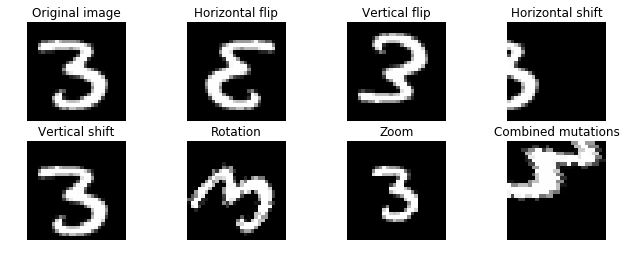
\includegraphics[height=7cm]{img/data_augmentation}
  \caption{Examples of augmented images}
\label{fig:augmented_images}
\end{figure}

As described in Chapter~\ref{sub:dl_drivers}, deep neural networks profit from
large amounts of data.
Therefore, the first step in reducing overfitting is usually to add
more data.
This can be achieved using either more real data, or by generating new examples
from already used training data.
This technique called \textit{data augmentation} is common in computer vision
problems that deal with images~\cite{Simard2003}.
It refers to the enhancement of training data with variations of existing training
examples.
For images these augmented images can created using minor mutations, e.g., random rotations, flips, shifts or
color changes.
Fig.~\ref{fig:augmented_images} shows examples of a handwritten character being
mutated in various ways.
Data augmentation leads to a bigger variety of inputs, which has been shown
to reduce overfitting for deep neural networks~\cite{Krizhevsky2012}.
